\documentclass{article}
\usepackage{tikz}
\usepackage[simplified]{pgf-umlcd}
\usepackage{multirow}
\usepackage{float}
\usetikzlibrary{arrows, arrows.meta}

\begin{document}

\title{
    Tarea 2 - Normalizacion del Modelo a 3FN \\
    INF239 - BASES DE DATOS
}
\author{
    Matías Peñaloza 202373037-8 \\
    Hans González 202373020-3
}
\date{
    2025-1
}
\maketitle


\section{Modelo Anterior (Forma Relacional)}
\begin{center}
\resizebox{1.1\textwidth}{!}{
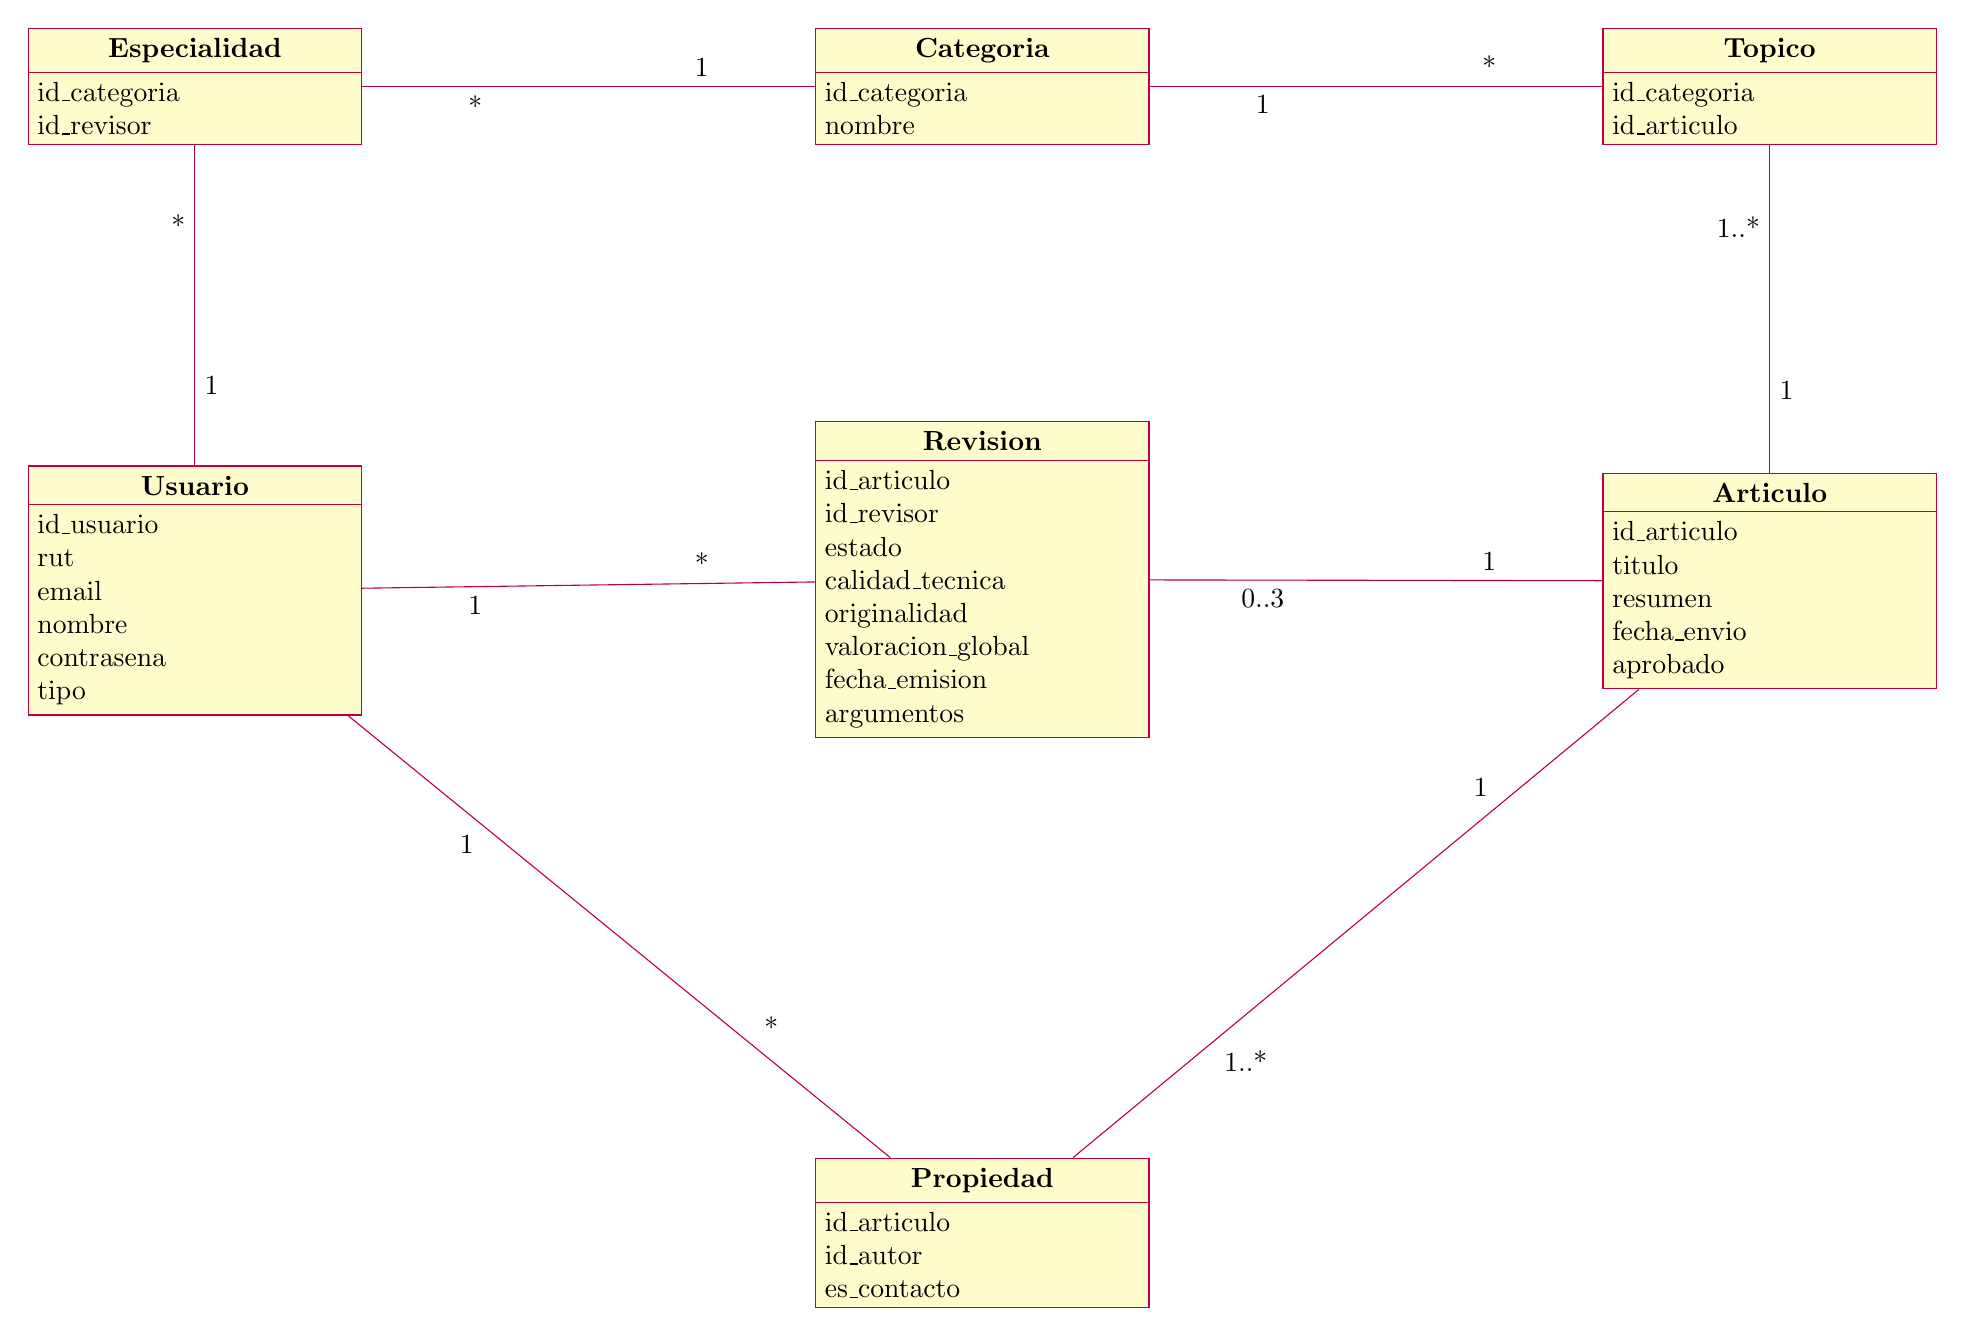
\begin{tikzpicture}
    
    \begin{class}[text width=4cm]{Categoria}{5, -5}
        \attribute{id\_categoria}
        \attribute{nombre}
    \end{class}
    
    \begin{class}[text width=4cm]{Topico}{15, -5}
        \attribute{id\_categoria}
        \attribute{id\_articulo}
    \end{class}
    
    \begin{class}[text width=4cm]{Especialidad}{-5, -5}
        \attribute{id\_categoria}
        \attribute{id\_revisor}
    \end{class}
    
    \begin{class}[text width=4cm]{Usuario}{-5, -10.56}
        \attribute{id\_usuario}
        \attribute{rut}
        \attribute{email}
        \attribute{nombre}
        \attribute{contrasena}
        \attribute{tipo}
    \end{class}

    \begin{class}[text width=4cm]{Articulo}{15, -10.65}
        \attribute{id\_articulo}
        \attribute{titulo}
        \attribute{resumen}
        \attribute{fecha\_envio}
        \attribute{aprobado}
    \end{class}
    
    \begin{class}[text width=4cm]{Revision}{5, -10}
        \attribute{id\_articulo}
        \attribute{id\_revisor}
        \attribute{estado}
        \attribute{calidad\_tecnica}
        \attribute{originalidad}
        \attribute{valoracion\_global}
        \attribute{fecha\_emision}
        \attribute{argumentos}
    \end{class}
    
    \begin{class}[text width=4cm]{Propiedad}{5, -19.35}
        \attribute{id\_articulo}
        \attribute{id\_autor}
        \attribute{es\_contacto}
    \end{class}
    
    \association{Propiedad}{}{1..*}{Articulo}{1}{}
    \association{Revision}{}{0..3}{Articulo}{1}{}
    \association{Topico}{}{1..*}{Articulo}{1}{}
    \association{Topico}{}{*}{Categoria}{1}{}
    \association{Especialidad}{}{*}{Categoria}{1}{}
    \association{Propiedad}{}{*}{Usuario}{1}{}
    \association{Revision}{}{*}{Usuario}{1}{}
    \association{Especialidad}{}{*}{Usuario}{1}{}
    
\end{tikzpicture}
}
\end{center}

\section{Proceso de Normalización}
\subsection{Vistas}
\begin{itemize}
    \item Articulo(id\_articulo, titulo, resumen, fecha\_envio, aprobado)
    \item Usuario(id\_usuario, rut, email, nombre, contrasena, tipo)
    \item Propiedad(id\_articulo, id\_autor, es\_contacto)
    \item Revision(id\_articulo, id\_revisor, estado, calidad\_tecnica, originalidad, valoracion\_global, fecha\_emision, argumentos)
    \item Topico(id\_categoria, id\_articulo)
    \item Especialidad(id\_categoria, id\_revisor)
    \item Categoria(id\_categoria, nombre)
\end{itemize}
\subsection{Primera Forma Normal (1FN)}
Eliminar grupos repetitivos.\\\\
NO HAY.

\subsection{Segunda Forma Normal (2FN)}
Eliminar dependencias parciales.\\\\
NO HAY.

\subsection{Tercera Forma Normal (3FN)}
Eliminar dependencias transitivas.\\\\
NO HAY.

\section{Cambios}
Ya que el modelo original ya estaba en 3FN, no se realizaron cambios significativos.
Unicamente se cambio el tamaño de \textbf{Usuario.contrasena} de 30 a 60 para ajustarlo al tamaño de una funcion de hash.

\end{document}